\chapter{ Computational Analysis}\label{chap:computational_analysis}

In this chapter,  computational aspects of the application are discussed.
 % This chapter introduces some specifications of the implementation of our solution.\\


  \section{ Autocorrelation function implementation}
    The autocorrelation function introduced in Equation \eqref{eq:4} can be
    implemented in several ways:

      \subsection{Naive approach}
        The naive approach for the autocorrelation function consists in
        compute all possible shifts of the sequence and then
        correlate them with the base sequence as shown in Figure
        \ref{naive_auto:fig:1}.  This algorithm is simple to implement and
        follows from the mathematical definition, however it is too slow. The
        correlation function for each component have to be computed, leading to a
        complexity of $O(n^{2})$, where $n$ is the length of the sequence. The
        overhead due to the building of  the shifted sequence weights on the
        performance. Some overhead could be avoided by using slice of the sequence
        but it will not affect the complexity.\\

      \subsection{Circular convolution theorem}\label{section:impl:convolution}
      We explore the properties of the autocorrelation function. The convolution theorem\cite{golomb_ref} gives a  direct relation between between the correlation function and the Discrete Fourier Transform (DFT)\\
      \begin{theorem}
          Given a sequence $S$ and its DFT, then
          \begin{equation}
            A(S) = DFT^{-1}[DFT\{S\} · DFT\{S\}^{*}]
          \end{equation}
          where $DFT\{S\}^{*}$ represents the complex conjugate of $DFT\{S\}$.
        \end{theorem}

        To compute the DFT and its inverse, the Fast Fourier
        Transform\cite{fast_fourier_transform} algorithm can be implemented. Then complexity is $O(n \log n)$.  However, now the types of the data change from integer in the naive approach to handle complex numbers. Then according to  property \ref{autocorrelation:prop:1}, it will always return the same type as the original sequence. This means that the operations are more computationally expensive due to operating with complex numbers instead of integers.
          \begin{figure}
            \inputpython{Chapters/Implementation/naive.py}{0}{100}
            \caption{An example implementation of the naive autocorrelation}
            \label{naive_auto:fig:1}
          \end{figure}

      \subsection{Composition method implementation}

      The previous discussion does not take into account the special structure of sequences generated by the composition method. It is possible to take advantage of some peculiarities to improve on the computation of the correlation.

     Taking advantage of Property \ref{composition:prop:1}, a faster algorithm can be designed. First of all, the complexity function of this new algorithm depends on the length of the shift sequence $m$  and the length of the base sequence $p$ with a complexity of $O(m^2 \log p)$. This means
      that when $m\log(p) < p\log(mp)$ this algorithm has a better complexity than the general approach.\\

      In addition, this method is more cache friendly too as the data source of the function is smaller and it
      does not need to use complex number operations in binary sequences. The biggest improvement in respect of the Fourier Transform approach is that to check for the partial autocorrelation, it is possible to do it without having to complete the computation of the whole autocorrelation function. This will be important for the brach and bound algorithm for the exhaustive search.\\

      An example implementation of this algorithm is shown in Figure
      \ref{composite_auto:fig:1}.

      \begin{figure}[ht!]
        \inputpython{Chapters/Implementation/composite.py}{0}{100}
        \caption{The Cython implementation of the autocorrelation for the composition method.}
        \label{composite_auto:fig:1}
      \end{figure}

  The complete implementation of the single thread branch and bound algorithm used
  in the project is shown in Figure \ref{composite_auto:fig:2}.

  \begin{figure}[ht!]
    \inputpython{Chapters/Implementation/branch_and_bound.py}{0}{100}
    \caption{A Cython implementation of the branch and bound algorithm. Notice
    the amount of extra boilerplate code to achive C performance.}
    \label{composite_auto:fig:2}
  \end{figure}


  \section{Parallelism model}

  For the parallelism of the project, it was decided to work with MPI (Message
  Passing Interface).  MPI is a library specification for message-passing, proposed
  as a de facto standard for parallel computing implementation. As the software
  will be deployed in a system with an interconnection network, a shared-memory
  parallelism would lead to a high latency in the assignation of tasks
  reducing performance. There are several implementations of MPI, many of which are
  open-source or in the public domain.\\

 From the available implementations, a pure
 Python one (MPI4PY\footnote{https://github.com/mpi4py/mpi4py}) was chosen based on
 the easiness of the development and its compatibility with different
 implementations of the MPI standard.\\

 For the purpose of this project, MPICH\footnote{https://www.mpich.org/} is used as
 the reference MPI implementation as the bindings of MPI4PY support it and it is the
 implementation used in the cluster we are working with\footnote{https://web.archive.org/web/20200823200600/https://www.ce.unican.es/resource/computing/}.\\

  In our particular problem, a set of tasks was defined to be
  distributed between the different nodes. This tasks are subtrees from the
  search space with a given height that defines the size of the task  see Figure
  \ref{tasks:fig:1} for an example. Due to different sizes of the tasks,  a static
  scheduler would not be efficient.\\


  \begin{figure}[ht!]
    \begin{center}
      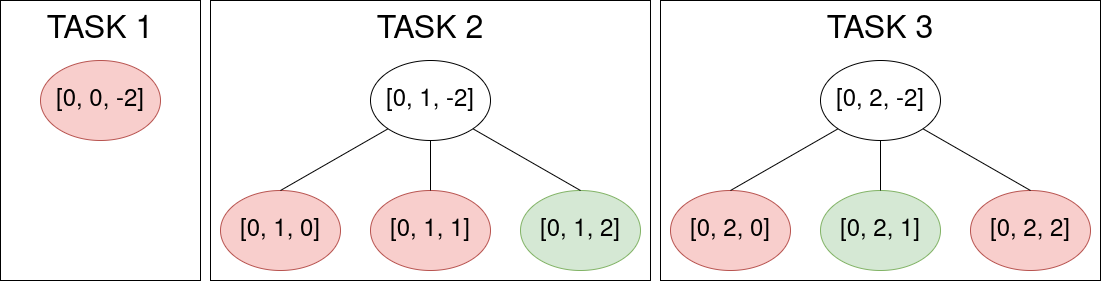
\includegraphics[scale=0.4]{Chapters/Implementation/Example_tasks.png}
    \end{center}
    \caption{An example distribution of tasks for the example at Figure
    \ref{bb:fig:1}.}
    \label{tasks:fig:1}
  \end{figure}

  The preliminary version of the software implemented this model.  However, if a branch is not pruned when assigning the tasks, there will still be an exponential number of tasks
 given by $p^{m-t}$ where $p$ is the length of the base sequence,$m$ is the
  length of the shift sequence  and $t$ is the task size.  If $t$ is close to $m$, the task balancer has to deal with a few remainding  task to asig, however it will not impact drastically the performance.\\

  A second version of the algorithm applies branch and bound to generate only candidates with good Hamming properties.
  This rules out all branches that would led to a bad resulting autocorrelation and would not generate any useful sequences. The code
  implementation is shown in Figures \ref{parallelism_example:fig:1} and
  \ref{parallelism_example:fig:2}.\\

  \begin{figure}[ht!]
    \inputpython{Chapters/Implementation/Example_parallelism_master.py}{0}{100}
    \caption{A Python implementation of the master proccess}
    \label{parallelism_example:fig:1}
  \end{figure}

  \begin{figure}[ht!]
    \inputpython{Chapters/Implementation/Example_parallelism_slave.py}{0}{100}
    \caption{A Python implementation of an slave proccess}
    \label{parallelism_example:fig:2}
  \end{figure}
